\documentclass{article}
\usepackage[utf8]{inputenc}
\usepackage[a4paper, margin=2.5cm]{geometry}
\usepackage{graphicx}
% \usepackage[french]{babel}

%\usepackage[default,scale=0.95]{opensans}
\usepackage[T1]{fontenc}
\usepackage{amssymb} %math
\usepackage{amsmath}
\usepackage{amsthm}
\usepackage{systeme}
\usepackage{fancyhdr}
\usepackage{subcaption}

\usepackage{hyperref}
\hypersetup{
    colorlinks=true,
    linkcolor=blue,
    filecolor=magenta,      
    urlcolor=cyan,
    pdftitle={Overleaf Example},
    % pdfpagemode=FullScreen,
    }
\urlstyle{same} %\href{url}{Text}

\theoremstyle{plain}% default
\newtheorem{thm}{Théorème}[section]
\newtheorem{lem}[thm]{Lemme}
\newtheorem{prop}[thm]{Proposition}
\newtheorem*{cor}{Corollaire}
%\newtheorem*{KL}{Klein’s Lemma}

\theoremstyle{definition}
\newtheorem{defn}{Définition}[section]
\newtheorem{exmp}{Exemple}[section]
% \newtheorem{xca}[exmp]{Exercise}

\theoremstyle{remark}
\newtheorem*{rem}{Remarque}
\newtheorem*{note}{Note}
%\newtheorem{case}{Case}

\title{
    Deep Learning Practical Work \\
    \Large \textbf{Basics on deep learning for vision}
}

\author{Aymeric \textsc{Delefosse} \& Charles \textsc{Vin}}
\date{2023 -- 2024}

\fancyhead{}
\fancyhead[L]{RDFIA}\fancyhead[R]{\textsc{DAC 2023 -- 2024}}
\pagestyle{fancy}
\thispagestyle{plain}

\begin{document}
\maketitle

\section{Introduction to neural networks}
\subsection{Theorical Foundation}
\subsubsection{Supervised dataset}
\paragraph{1. $\bigstar$ What are the train, val and test sets used for?}
The training dataset is utilized to train the model, while the test dataset is employed to assess the model's performance on previously unseen data. Lastly, the validation set constitutes a distinct subset of the dataset employed for the purpose of refining and optimizing the model's hyperparameters.

\paragraph{2. What is the influence of the number of exemples $N$?}
A larger number of examples can enhance the model's capacity to generalize and improve its robustness against noise or outliers. Conversely, a smaller number of examples can make the model susceptible to overfitting. It is important to note that increasing the dataset size can also lead to an escalation in the computational complexity of the model training process.

\subsubsection{Network architecture}
\paragraph{3. Why is it important to add activation functions between linear transformations?}
Otherwise, we would simply be aggregating linear functions, resulting in a linear output. Activation functions introduce non-linearity to the network, enabling the model to capture and learn more intricate patterns than those achievable through linear transformations alone.

\paragraph{4. $\bigstar$ What are the sizes $n_x$, $n_h$, $n_y$ in the figure 1? In practice, how are these sizes chosen?}
\begin{itemize}
    \item $n_x = 2$ represents the input size (data dimension).
    \item $n_h = 4$ represents the hidden layer size, selected based on the desired complexity of features to be learned in the hidden layer. An excessively large size can result in overfitting.
    \item $n_y = 2$ represents the output size, determined according to the number of classes in $y$.
\end{itemize}

\paragraph{5. What do the vectors $\hat{y}$ and $y$ represent? What is the difference between these two quantities?}
$y \in \{0,1\}$ represents the ground truth, where the values are binary (0 or 1).
$\hat{y} \in [0,1]$ represents a probability-like score assigned to each class by the model. $\hat{y}$ reflects the model's level of confidence in its predictions for each class.

\paragraph{6. Why use a $\text{SoftMax}$ function as the output activation function?}
The reason for employing the SoftMax function is to transform $\tilde{y} \in \mathbb{R}$ into a probability distribution. While there are several methods to achieve this transformation, $\text{SoftMax}$ is a commonly utilized choice, especially in multi-class classification problems.

\paragraph{7. Write the mathematical equations allowing to perform the \textit{forward} pass of the neural network, i.e. allowing to successively produce $\hat{h}$, $ h $, $ \tilde{y} $, $ \hat{y} $, starting at $x$.}
Let $W_i$ and $b_i$ denote the parameters for layer $i$, $f_i(x) = x W_i ^T + b_i$ represent the linear transformation, and $g_i(x)$ be the activation function for layer $i$.

Calculate the weighted sum and activation for the first hidden layer:
\begin{align*}
    \tilde{h} & = f_0(x)         \\
    h         & = g_0(\tilde{h})
\end{align*}

Proceed to the output layer by computing the weighted sum and activation for the output layer:
\begin{align*}
    \tilde{y} & = f_1(h)         \\
    \hat{y}   & = g_1(\tilde{y})
\end{align*}

These equations describe the sequential steps involved in the forward pass of the neural network, ultimately producing the output $\hat{y}$ based on the input $x$.

\subsection{Loss function}
\paragraph{8. During training, we try to minimize the loss function. For cross entropy and squared error, how must the $ \hat{y}_i $  vary to decrease the global loss function $ \mathcal{L} $?}
Our aim is to minimize the loss function $\mathcal{L}$ to train a model effectively. To decrease cross-entropy loss, make $\hat{y}_i$ closer to 1 when $y_i$ is 1 and closer to 0 when $y_i$ is 0.

For the cross-entropy loss, $\hat{y}_i$ should vary in a way that makes it closer to the true target value $y_i$ for each data point. Specifically, when $y_i = 1$, $\hat{y}_i$ should be pushed towards 1. The closer $\hat{y}_i$ is to 1, the lower the loss. Conversely, when $y_i = 0$, $\hat{y}_i$ should be pushed towards 0. The closer $\hat{y}_i$ is to 0, the lower the loss.

For squared error loss, $\hat{y}_i$ should vary in a way that makes it closer to the true target value $y_i$ for each data point. The goal is to minimize the squared difference between $\hat{y}_i$ and $y_i$. This means that if $\hat{y}_i$ is greater than $y_i$, it should decrease, and if $\hat{y}_i$ is smaller than $y_i$, it should increase.

\paragraph{9. How are these functions better suited to classification or regression tasks?}
Cross-entropy loss is better suited for classification tasks for several reasons:

\begin{itemize}
    \item Cross-entropy loss is based on the negative logarithm of the predicted probability of the true class. This logarithmic nature amplifies errors when the predicted probability deviates from 1 (for the correct class) and from 0 (for incorrect classes), depicted in Figure~\ref{CELoss}. Consequently, it effectively penalizes misclassifications, making it particularly suitable for classification tasks. However, it is imperative that $\hat{y}$ remains within the range $[0, 1]$ for this loss to be effective.
    \item Cross-entropy loss is often used in conjunction with the SoftMax activation function in the output layer of neural networks for multi-class classification. The SoftMax function ensures that the predicted probabilities sum to 1, aligning perfectly with the requirements of the cross-entropy loss.
\end{itemize}

\begin{figure}[!htbp]
    \centering
    \includegraphics*[width=0.6\textwidth]{figs/cross_entropy.png}
    \label{CELoss}
\end{figure}

On the other hand, Mean Squared Error serves a different role and is better suited for regression tasks:

\begin{itemize}
    \item MSE is ideal when dealing with $(y, \hat{y}) \in \mathbb{R}^2$ (as opposed to the bounded interval $[0, 1]$).
    \item MSE is advantageous due to its convexity, which simplifies optimization. However, it's important to note that it may not always be the best choice for every regression task, especially when dealing with outliers, as it can be sensitive to extreme values.
\end{itemize}

\newpage
\subsection{Optimization algorithm}
\paragraph{10. What seem to be the advantages and disadvantages of the various variants of gradient descent between the classic, mini-batch stochastic and online stochastic versions? Which one seems the most reasonable to use in the general case?}
Gradient computation becomes computationally expensive as it scales with the number of examples included. However, including more examples enhances gradient exploration with precision and stability, analogous to the exploration-exploitation trade-off in reinforcement learning.

Classic gradient descent offers stability, particularly with convex loss functions, featuring deterministic and reproducible updates. Nonetheless, its stability may lead to getting trapped in local minima when dealing with non-convex loss functions. Additionally, it is computationally intensive, especially for large datasets, as it demands evaluating the gradient with the entire dataset in each iteration.

Mini-Batch Stochastic Gradient Descent (SGD) converges faster compared to classic gradient descent by updating model parameters with small, random data subsets (mini-batches). This stochasticity aids in escaping local minima and exploring the loss landscape more efficiently. However, it may introduce noise and oscillations.

On the other hand, Online Stochastic Gradient Descent offers extremely rapid updates, processing one training example at a time, making it suitable for streaming or large-scale online learning scenarios. However, its highly noisy updates can result in erratic convergence or divergence, necessitating careful learning rate tuning.

For training deep neural networks in the general case, mini-batch stochastic gradient descent is the most reasonable choice. It strikes a balance between the computational efficiency of classic gradient descent and the noise resilience and convergence speed of online SGD.

\paragraph{11. $\bigstar$ What is the influence of the \textit{learning rate} $\eta$  on learning?}
The learning rate plays a crucial role in influencing various aspects of the learning process, including convergence speed, stability, and the quality of the final model.

A higher learning rate typically results in faster convergence because it leads to larger updates in model parameters during each iteration. However, an excessively high learning rate can cause issues such as overshooting, where the optimization process diverges or oscillates around the minimum, preventing successful convergence.

Conversely, a smaller learning rate allows the optimization algorithm to take smaller steps, which can be advantageous for exploring local minima more thoroughly and escaping shallow local minima. Nonetheless, if the learning rate is too small, it may lead to slow convergence or getting stuck in local minima.

To address these challenges, various techniques like learning rate schedules (gradually reducing the learning rate over time) or adaptive learning rate methods (e.g., Adam) have been developed to automate learning rate adjustments during training. The choice of learning rate may also be influenced by the batch size used in mini-batch stochastic gradient descent, as smaller batch sizes may require smaller learning rates to maintain stability.

In practice, selecting an appropriate learning rate often involves experimentation and can be problem-specific. Techniques such as grid search or random search, in combination with cross-validation, can aid in determining an optimal learning rate for a particular task.

\paragraph{12. $\bigstar$ Compare the complexity (depending on the number of layers in the network) of calculating the gradients of the \textit{loss} with respect to the parameters, using the naive approach and the \textit{backprop} algorithm.}
The naive method involves calculating the gradient of the loss function with respect to each parameter independently, without leveraging the computational advantages of knowing the derivatives' interdependencies across layers. For a network with a large number of parameters, this is computationally expensive and inefficient, essentially repeating a substantial amount of calculation needlessly. The complexity becomes substantial as the number of layers (and, as a result, the number of parameters) increases. It becomes a combinatorial problem.

Backpropagation is a far more efficient strategy due to its intrinsic use of the chain rule from calculus to 'remember' past calculations. This technique essentially breaks down the full problem of calculating a derivative on a complex, multi-stage function into smaller, more manageable pieces. Then, it smartly recombines these pieces, significantly reducing computational redundancy. This methodology dramatically reduces the number of computations, particularly for networks with a large number of interconnected layers and parameters.

\paragraph{13. What criteria must the network architecture meet to allow such an optimization procedure?}
For the backpropagation algorithm to be applicable, several criteria must be met. First of all, each layer function, including the activation functions and the loss function, must be differentiable with respect to their parameters. This is crucial for calculating gradients during the training process. Furthermore, as backpropagation relies on the sequential flow of information from the input layer to the output layer, the network architecture should possess a feedforward, sequential structure without loops or recurrent connections. Loops or recurrent connections can introduce complications in gradient calculations.

\paragraph{14. The function SoftMax and the \textit{loss} of \textit{cross-entropy} are often used together and their gradient is very simple. Show that the \textit{loss} can be simplified by:
    \[l = - \sum_{i}^{} y_i \tilde{y}_i + \log_{} (\sum_{i}^{} e^{\tilde{y}_i}).\]}
Let us define the cross-entropy loss as \( l(y, \hat{y}) = - \sum_{i=1}^{N} y_i \log \hat{y}_i \), where \( N \) represents the total number of examples. The SoftMax function for a vector \( \tilde{y} \in \mathbb{R}^D \) is defined as \( \text{SoftMax}(\tilde{y_i}) = \frac{e^{\tilde{y_i}}}{\sum_{j=1}^{D} e^{\tilde{y_j}}} \). Notably, the output of the SoftMax function serves as the input for the cross-entropy loss, denoted as \( \hat{y}_i = \text{SoftMax}(\tilde{y_i}) \). Let us substitute this value into the expression.

\begin{align*}
    l(y, \hat{y}) & = - \sum_{i=1}^{N} y_i \log_{} \hat{y}_i                                                                \\
                  & = - \sum_{i=1}^{N} y_i \log_{} \text{SoftMax}(\tilde{y_i})                                              \\
                  & = - \sum_{i=1}^{N} y_i \log_{} \frac{e^{\tilde{y_i}}}{\sum_{j=1}^{D} e^{\tilde{y_j}} }                  \\
                  & = - \sum_{i=1}^{N} y_i \left[ \log_{} e^{\tilde{y}_i} - \log_{} \sum_{j=1}^{D} e^{\tilde{y}_j}  \right] \\
                  & = - \sum_{i=1}^{N} y_i \tilde{y}_i - y_i \log_{} \sum_{j=1}^{D}e^{\tilde{y}_j}                          \\
                  & = - \sum_{i=1}^{N} y_i \tilde{y}_i + \sum_{i=1}^{N} y_i \log_{} (\sum_{j}^{D}e^{\tilde{y}_j}) \\
                  & = - \sum_{i=1}^{N} y_i \tilde{y}_i + \log_{} (\sum_{j}^{D}e^{\tilde{y}_j}) \sum_{i=1}^{N} y_i 
\end{align*}

Since $y_i$ is One Hot encoded we know that $\sum_i y_i = 1$. Thus, we have the final expression for the cross-entropy loss:

$$ l(y, \hat{y}) = - \sum_{i}^{} y_i \tilde{y}_i + \log_{} \left(\sum_{i}^{} e^{\tilde{y}_i}\right) $$

\paragraph{15. Write the gradient of the \textit{loss} (\textit{cross-entropy}) relative to the intermediate output $ \tilde{y} $ }
\begin{align*}
    \frac{\partial l}{\partial \tilde{y}_i} & = -y_i + \frac{\frac{\partial }{\partial \tilde{y}_i } (\sum_{j=1}^{N} e^{ \tilde{y}_j })}{\sum_{j=1}^{N} e^{ \tilde{y}_j }} \\
                                            & = - y_i + \frac{e^{\tilde{y}_i}}{\sum_{j=1}^{n_y} e^{ \tilde{y}_j}}                                                          \\
                                            & = - y_i + \text{SoftMax}(\tilde{y})_i
\end{align*}
\[
    \nabla _{\tilde{y}}l = \begin{pmatrix}
        \frac{\partial l}{\partial \tilde{y}_1} \\
        \vdots                                  \\
        \frac{\partial l}{\partial \tilde{y}_{n_y}}
    \end{pmatrix} = \begin{pmatrix}
        \text{SoftMax}(\tilde{y})_1 - y_1 \\
        \vdots                            \\
        \text{SoftMax}(\tilde{y})_{n_y} - y_{n_y}
    \end{pmatrix} \\
    = \hat{y} - y
    .\]

\paragraph{16. Using the \textit{backpropagation}, write the gradient of the \textit{loss} with respect to the weights of the output layer $ \nabla _{W_y}l $ . Note that writing this gradient uses $ \nabla _{\tilde{y}}l $ . Do the same for $ \nabla _{b_y}l $.}

Starting with \( \nabla _{W_y} l \), we have:

\[
    \frac{\partial l}{\partial W_{y,ij}} = \sum_{k}^{} \frac{\partial l}{\partial \tilde{y}_k} \frac{\partial \tilde{y}_k}{\partial W_{y,ij}}
\]

This can be expressed as a matrix:

\[
    \nabla_{W_y} l = \begin{pmatrix}
        \frac{\partial l}{\partial W_{y, 1,1}}   & \dots  & \frac{\partial l}{\partial W_{y, 1,n_h}}    \\
        \vdots                                   & \ddots & \vdots                                      \\
        \frac{\partial l}{\partial W_{y, n_y,1}} & \dots  & \frac{\partial l}{\partial W_{y, n_y, n_h}}
    \end{pmatrix}
\]

First, let's compute $ \tilde{y}_k $
\begin{align*}
    \tilde{y}   & = h W_y^T + b^y                                                                                                                                  \\
                & = \begin{pmatrix}
                        h_{1} & \dots & h_{n_h}
                    \end{pmatrix} * \begin{pmatrix}
                                        W_{1, 1}   & \dots  & W_{1, n_y}   \\
                                        \vdots     & \ddots & \vdots       \\
                                        W_{n_h, 1} & \dots  & W_{n_h, n_y} \\
                                    \end{pmatrix} + \begin{pmatrix}
                                                        b^y_1 & \dots & b^y_{n_y}
                                                    \end{pmatrix}                                                                                      \\
                & = \begin{pmatrix}
                        \sum_{j=1}^{n_h} W^y_{1,j} h_{j} + b^y_1 & \sum_{j=1}^{n_h} W^y_{2,j} h_{j} + b^y_2 & \dots & \sum_{j=1}^{n_h} W^y_{n_h,j} h_{k,j} + b^y_{n_h}
                    \end{pmatrix} & \in \mathbb{R}^{1 \times n_h} \\
    \tilde{y}_k & = \sum_{j=1}^{n_h} W^y_{k,j} h_{j} + b_k^y, k \in [1, n_h]
\end{align*}

With this expression, we can now proceed with the calculation of the partial derivative of \( \tilde{y}_k \) with respect to \( W^y_{ij} \):

\[
    \frac{\partial \tilde{y}_k }{\partial W^y_{ij}} = \begin{cases}
        h_j & \text{ if } i=k   \\
        0   & \text{ otherwise}
    \end{cases}
\]

Now, we need to find \( \frac{\partial l}{\partial \tilde{y}_k} \). From the previous question, we have:

\[
    \frac{\partial l}{\partial \tilde{y}_k} = -y_k + \text{SoftMax}(\tilde{y})_k = \hat{y}_k - y_k
\]

Now, combining these results:

\[
    \frac{\partial l}{\partial W_{i,j}^y} = \sum_{k=1}^{n_h} \frac{\partial l}{\partial \tilde{y}_k} \frac{\partial \tilde{y}_k}{\partial W_{i,j}^y} =  \frac{\partial l}{\partial \tilde{y}_i} \frac{\partial \tilde{y}_i}{\partial W_{i,j}^y} = (\hat{y}_i - y_i) h_j = (\nabla _{W_y} l)_{i,j}
\]

So, the gradient of the loss with respect to the weights of the output layer \( \nabla_{W_y} l \) is given by \( \nabla _{\tilde{y}} ^T h \).

\begin{align*}
    \nabla_{W_y} l & = \begin{pmatrix}
                           \frac{\partial l}{\partial W^y_{1,1}}   & \dots  & \frac{\partial l}{\partial W^y_{1,n_h}}    \\
                           \vdots                                  & \ddots & \vdots                                     \\
                           \frac{\partial l}{\partial W^y_{n_y,1}} & \dots  & \frac{\partial l}{\partial W^y_{n_y, n_h}}
                       \end{pmatrix} \\
                   & = \begin{pmatrix}
                           (\hat{y}_1 - y_1) h_{1}         & \dots  & (\hat{y}_1 - y_1) h_{n_h}         \\
                           \vdots                          & \ddots & \vdots                            \\
                           (\hat{y}_{n_y} - y_{n_y}) h_{1} & \dots  & (\hat{y}_{n_y} - y_{n_y}) h_{n_h}
                       \end{pmatrix}                  \\
                   & = \begin{pmatrix}
                           \hat{y}_1 - y_1 \\
                           \vdots          \\
                           \hat{y}_{n_y} - y_{n_y}
                       \end{pmatrix} \begin{pmatrix}
                                         h_1 & h_2 & \dots & h_{n_h}
                                     \end{pmatrix}                                                     \\
                   & = \nabla _{\tilde{y}} ^T h
\end{align*}


% For the gradient with respect to the biases of the output layer \( \nabla_{b_y} l \), the calculation would be similar but would involve the derivative of \( \tilde{y}_k \) with respect to \( b_k^y \), which would be 1, and the gradient \( \frac{\partial l}{\partial \tilde{y}_k} \) remains the same. Putting it all together:

% \[
% \frac{\partial l}{\partial b_k^y} = \sum_{k=1}^{n_h} \frac{\partial l}{\partial \tilde{y}_k} \frac{\partial \tilde{y}_k}{\partial b_k^y} = (\hat{y}_k - y_k) \cdot 1 = \hat{y}_k - y_k
% \]

\paragraph{17. $\bigstar$ Compute other gradients : $ \nabla _{\tilde{h}} l, \nabla _{W_h} l, \nabla_{b_h}l $ }

\begin{enumerate}
    \item The gradient of the loss with respect to \( \tilde{h} \) can be computed using the chain rule:
    \[
        \frac{\partial l}{\partial \tilde{h}_i} = \sum_{k}^{} \frac{\partial l}{\partial h_k} \frac{\partial h_k}{\partial \tilde{h}_i} 
    .\]
    Let's compute those two terms
    \begin{itemize}
        \item 
        \[
            \frac{\partial h_k}{\partial \tilde{h}_i} = \frac{\partial \tanh (\tilde{h_k})}{\partial \tilde{h_i}} = \begin{cases}
            1 - \tanh^2 (\tilde{h_i}) = 1 - h_i^2 &\text{ if } k = i\\
            0 &\text{ otherwise}\\
        \end{cases} 
    .\]
    
    \item Having $ \tilde{y}_i = \sum_{j=1}^{n_h} W_{i,j}^y h_j +b_i^y$ in mind and recovering $ \frac{\partial l}{\partial \tilde{y}_i} = \hat{y}_i - y_i = \delta ^y_i $ from past question.
    \[
        \frac{\partial l}{\partial h_k} = \sum_{j=1}^{} \frac{\partial l}{\partial \tilde{y_j}} \frac{\partial \tilde{y}_j}{\partial h_k} = \sum_{j=1}^{} \delta ^y_j W^y_{j,k}
    .\]
    \end{itemize}
    Finaly we have 
    \begin{align*}
        \frac{\partial l}{\partial \tilde{h}_i} &= \sum_{k}^{} \frac{\partial l}{\partial h_k} \frac{\partial h_k}{\partial \tilde{h}_i}  \\ 
        &= \sum_{k}^{} (\sum_{j}^{} \delta ^y_j W^y_{j,k}) \times \begin{cases}
            1 - h_i^2 &\text{ if } k = i\\
            0 &\text{ otherwise}\\
        \end{cases} \\
        &= (1 - h_i^2) (\sum_{j}^{} \delta ^y_j W^y_{j,i}) \\
        &= \delta ^h _i     
    \end{align*}
    So, the gradient \( \nabla _{\tilde{h}} l \) is a vector with elements $ \delta ^h _i $ 

    \[
        \nabla _{\tilde{h}} l = (1 - h^2) \odot (\nabla _{\tilde{y}} l * W^y)
    .\]


    \item $ \nabla _{W^h} l $ is a matrix composed of elements 
    \[
        \frac{\partial l}{\partial W^h _{i,j}} = \sum_{k}^{} \frac{\partial l}{\partial \tilde{h}_k} \frac{\partial \tilde{h}_k}{\partial W^h_{i,j}} 
    .\]
    From the previous question we already have $ \frac{\partial l}{\partial h_k} = (1 - h_k^2) (\sum_{j}^{} \delta ^y_j W^y_{j,k}) = \delta_k^h$. So let's compute the other term $ \frac{\partial \tilde{h}_k}{\partial W^h_{i,j}}  $ from $ \tilde{h}_k = \sum_{j=1}^{n_x} W^h_{k,j} x_j + b_k^h $ 
    
    \[
        \frac{\partial \tilde{h}_k}{\partial W^h_{i,j}} = \begin{cases}
            x_j &\text{ if } k = i\\
            0 &\text{ otherwise }\\
        \end{cases} 
    .\]
    So \begin{align*}
        \frac{\partial l}{\partial W^h _{i,j}} &= \sum_{k}^{} \frac{\partial l}{\partial \tilde{h}_k} \frac{\partial \tilde{h}_k}{\partial W^h_{i,j}} \\
            &= \sum_{k}^{}\delta ^h_k \times \begin{cases}
                x_j &\text{ if } k = i\\
                0 &\text{ otherwise }\\
            \end{cases} \\
            &= \delta _i^h x_j \\
        \nabla _W^h &= \nabla _{\tilde{h}} ^T l * x
    \end{align*}


    \item Last but not least 
    \[
        \frac{\partial l}{\partial b_i^j} = \sum_{k}^{} \frac{\partial l}{\partial \tilde{h}_k} \frac{\partial \tilde{h}_k}{\partial b_i^h} = \sum_{k}^{}\delta _k^h * \begin{cases}
            1 &\text{ if } k = i\\
            0 &\text{ else}\\
        \end{cases} = \delta ^h_i
    .\]
    
    \[
        \nabla _{b^h} = \nabla _{\tilde{h}} l
    .\]
    
\end{enumerate}

\newpage
\section{Introduction to convolutional networks}
\subsection{Questions}
\paragraph{1. Considering a single convolution filter of padding $p$, stride $s$ and kernel size $k$, for an input of size $x \times y \times z$ what will be the output size?
How much weight is there to learn?
How much weight would it have taken to learn if a fully-connected layer were to produce an output of the same size?} 
Let's note $x_{\text{out}}, y_{\text{out}}, z_{\text{out}}$ our output size. Then, given a convolution filter of padding $p$, stride $s$ and kernel size $k$:

\begin{align}
    \label{eq:1} x_{\text{out}} = \frac{x + 2 \times p - k}{s} + 1 \\
    \label{eq:2} y_{\text{out}} = \frac{y + 2 \times p - k}{s} + 1 \\
    \label{eq:3} z_{\text{out}} = \frac{z + 2 \times p - k}{s} + 1 
\end{align}

We have a single convolution filter. Given our kernel of size $ k \times k $, we thus have $ 1 \times k \times k = k^2 $ weights to learn. In a fully-connected layer, we would have $(x \times y \times z \times k^2)$ weights to learn.

\paragraph{2. $ \bigstar $ What are the advantages of convolution over fully-connected layers? What is its main limit?}
Using fully-connnected layers with image involved \textit{a lot} of parameters, each for one pixel of the image. Fully-connected layer are also sensitive to variance in image even a simple translation.

From the other side, convolutionnal layer solve those problems. Using convolution with a shared set of weight (for the filter/kernels) accross the entire input permit to learn and detect \textit{local} spacial patterns/features at different locations. Convolutionnal layer also have the ability to hierachicly combine features. The lower layers capture low-level features like edges and textures, while the higher layers capture more complex features and object representations.

The limit is that convolutional layers lack of global context and focus primaly on local patterns. It's hard for them to understand relationships between distant parts of the input, which can be important in some applications.

\paragraph{3. $ \bigstar $ Why do we use spatial pooling?}
Spatial pooling permit to gain in invariance, especialy translation. By summarizing a local region with a pooled value, the precise location of the feature becomes less important. It's a form of regularization by selecting the most relevant information.

Polling also permit a dimensionality reduction by reducing spatial dimensions of the outputing feature map. This dimensionality reduction significantly decreases the computational cost of subsequent layers.

Max and average polling layer are the most used polling layers. Max pooling helps in achieving translation invariance and reducing spatial dimensions. It is effective in preserving the most important features in the input data. Average pooling also reduces spatial dimensions and helps in achieving translation invariance. It can be less sensitive to outliers in the input data compared to max pooling.

\paragraph{4. $ \bigstar $ Suppose we try to compute the output of a classical convolutional network for an input image larger than the initially planned size. Can we (without modifying the image) use all or part of the layers of the network on this image?}
% By definition, a convolution layer does not dependent of the size of the input, it will take the image, do convolution on it till the end of the image, and output another image. So when staking convolution and pooling layer (which do a convolution too), the output size is only dependent from the input size. In some other words, the input size of the image is not a hyperparameter of the convolution layer.

% In a classical convolutional network, this output from the stacking of convolutionnal and pooling layers is flattened to become the input of a fully-connected layer. The size of the flattened vector is dependent of the size of the outputed image from the convolution layers.

% But this time, we need to know the size of the input of our fully-connected layer in advance to set it up (like to initialse the parameters, ...).

% So when using an input image larger than the initially planned size, everything will run until the use of a fully connected layer because it expect a fixed size input. 
Inherent in its design, a convolution layer in a convolutional network is size-agnostic regarding its input; it simply performs convolutions across the entire span of the input image and outputs a correspondingly altered image. Sequentially, when convolution and pooling layers are stacked together, the resulting output size is purely a function of the input size. To rephrase, the input size of the image is not a critical hyperparameter for the convolution layer.

Within the conventional architecture of a convolutional network, the output derived from successive convolutional and pooling layers is typically 'flattened' to form the input for a subsequent fully-connected layer. Crucially, the size of this flattened vector is contingent on the size of the image output from the preceding convolution layers.

The challenge arises when we involve fully connected layers, as their initialization requires a priori knowledge of their input size to properly set up parameters such as weights. Consequently, when an input image is larger than initially planned, the network can operate normally up to the point of the fully connected layer(s), which anticipate input of a predetermined, fixed size.

\paragraph{5. Show that we can analyze fully-connected layers as particular convolutions.}
In a fully-connected layer, we associate one pixel of the flattened image too on weight. Both the weight and the flattened image are vector. But if we take the weights rearrange them into a matrix of the shape of the image, we can direclty do a term by term multiplication between this matrix and the image. Which is kind of a one slide convolution ! 

This $1 \times 1$ convolution use a stride equal to the width of the input image so that the filter doesn't slide to other positions. And has the filter size is exactly the same size as the image. The number of filter is equivalent to the number of neurons in the fully-connected layer.

\paragraph{6. Suppose that we therefore replace fully-connected by their equivalent in convolutions, answer again the question 4. If we can calculate the output, what is its shape and interest?}
\textbf{Not sure : }
%%%%%%%%%%%%%%%%%%%%%
For me, as with the fully connected layer,  we still have to know the input size to fix the filter size and the stride ahead. So it will still not work.
%%%%%%%%%%%%%%%%%%%%% A VERIFIER 

\paragraph{7. We call the receptive field of a neuron the set of pixels of the image on which the output of this neuron depends. What are the sizes of the receptive fields of the neurons of the first and second convolutional layers? Can you imagine what happens to the deeper layers? How to interpret it?}

\subsection{Training \textit{from scratch} of the model}
\subsubsection{Network architecture}
\paragraph{8. For convolutions, we want to keep the same spatial dimensions at the output as at the input. What padding and stride values are needed?}
We want $ x = x_{out}, y = y_{out} $: let's use our equations \ref{eq:1}, \ref{eq:2}, \ref{eq:3} to find the values of $p$ and $s$.
\[
    p = \frac{(s-1)x + k - s}{2}
.\]
Knowing $k = 5$ and that our images are of size $32 \times 32 $, we can pick any $p = \frac{31s - 27}{2}$. Because we generally want to use every pixel (and not padding pixels) so we pick $ s = 1 $ so $ p = 2 $ to minimise them both.


\paragraph{9. For max poolings, we want to reduce the spatial dimensions by a factor of 2. What padding and stride values are needed?} 
A pooling layer acts like a convolution: let's proceed as in question 8. This time we want $ x_{out} = \frac{1}{2}x, y_{out} = \frac{1}{2}y$.
\[
    p = \frac{(\frac{1}{2}s - 1) x + k - s}{2}
.\]
Knowing $k = 2$ and that our images are of size $32 \times 32 $, we can pick any $p = \frac{15s - 30}{2}$. We generally want to use every pixel (and not padding pixels) so we pick $ s = 2 $ so $ p = 0 $ to minimise them both.

\paragraph{10. $ \bigstar $ For each layer, indicate the output size and the number of weights to learn. Comment on this repartition.}
To make things easier, we made a plot of the CNN in figure \ref{AlexNetstylelog}. As you can see we are starting from a 3 channel image of 32 per 32 pixels. As question 8 and 9 suggest, convolution layers keep the same spatial dimension at the outpus as the input and pooling layers reduce the spatial dimensions by two. 
Here is the number of parameters : 
\begin{itemize}
    \item conv1: 32 filters of 5 by 5 for 3 channels $\rightarrow 32\times 5\times 5\times 3 = 2,400$ parameters
    \item conv2: 64 filters of 5 by 5 for 32 channels $\rightarrow 64\times 5\times 5\times 32 = 51,200$ parameters
    \item conv3: 64 filters of 5 by 5 for 64 channels $\rightarrow 64\times 5\times 5\times 64 = 102,400$ parameters
    \item 1000 neurons with a 1024 values as input $\rightarrow (1000 + 1)\times 1024=1,025,024$ parameters. The "$+1$" is for biases.
    \item 10 neurons with a 1000 values as input $\rightarrow 11\times 1000=11,000$ parameters
\end{itemize}
%%%%%%%%%%%%%%%%
% IL Y A DES BIAIS AUSSI DANS LES CONV A INCLURE DANS LES CALCULS
% https://stackoverflow.com/questions/42786717/how-to-calculate-the-number-of-parameters-for-convolutional-neural-network
%%%%%%%%%%%%%%%
% \begin{figure}[!htbp]
%     \centering
%     \includegraphics*[width=\textwidth]{figs/AlexNet_style.png}
%     \caption{}
%     \label{AlexNetstyle}
% \end{figure}
\begin{figure}[!htbp]
    \centering
    \includegraphics*[width=\textwidth]{figs/AlexNet_style_log.png}
    \caption{Network architecture}
    \label{AlexNetstylelog}
\end{figure}


\paragraph{11. What is the total number of weights to learn? Compare that to the number of examples.}
It makes a total of $ 1,192,024 $ parameters to train with 60,000 (6,000 images per class). It should be ok.
%%%%%%%%%%%%%%%%
% IS IT OK ?????
%%%%%%%%%%%%%%%%

\paragraph{12. Compare the number of parameters to learn with that of the BoW and SVM approach.}
De quoi il parle ??? feur

\subsubsection{Network learning}
\paragraph{14. $ \bigstar $ In the provided code, what is the major difference between the way to calculate loss and accuracy in train and in test (other than the the difference in data)?}
The difference here in the code is that we don't give an optimizer to \textit{epoch()} and so we do not train the network on test examples. There is no backward of the loss.
% Le code de base compute la loss à chaque batch, alors qu'on change les paramètres à chaque batch, donc ça rend les comparaisons plus difficile. En général (et c'est ce que j'ai changé dans le code), on compure la los

\paragraph{16. $ \bigstar $ What are the effects of the learning rate and of the batch-size?}
\begin{figure*}
    \centering
    \begin{subfigure}[b]{0.475\textwidth}
        \centering
        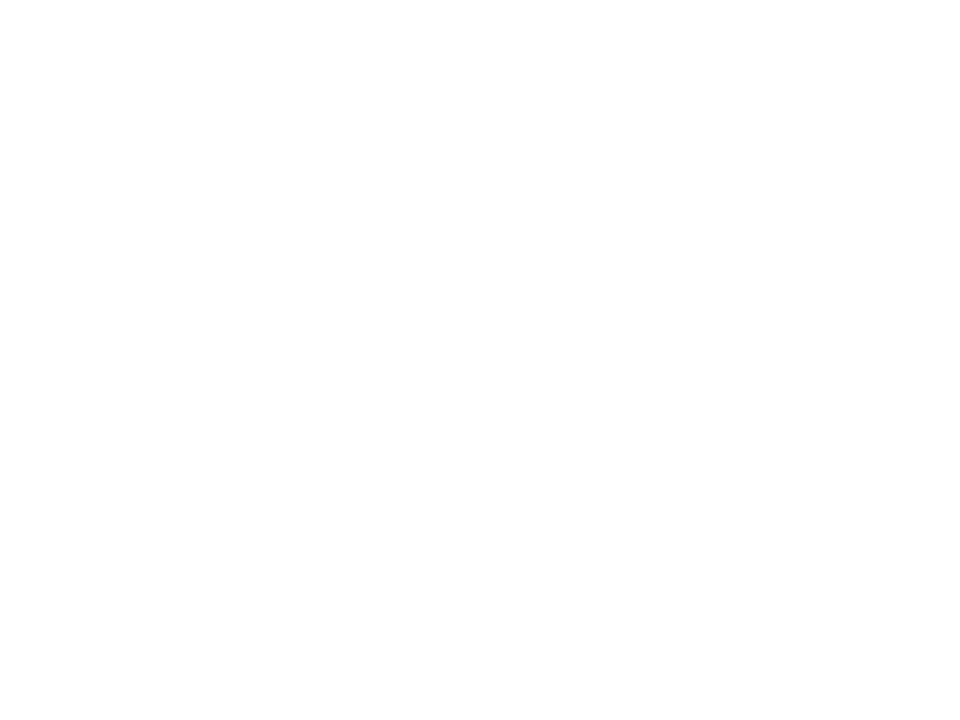
\includegraphics[width=\textwidth]{figs/batch32_lr0.1.pdf}
        \caption[Network2]%
        {{\small Network 1}}    
        \label{fig:mean and std of net14}
    \end{subfigure}
    \hfill
    \begin{subfigure}[b]{0.475\textwidth}  
        \centering 
        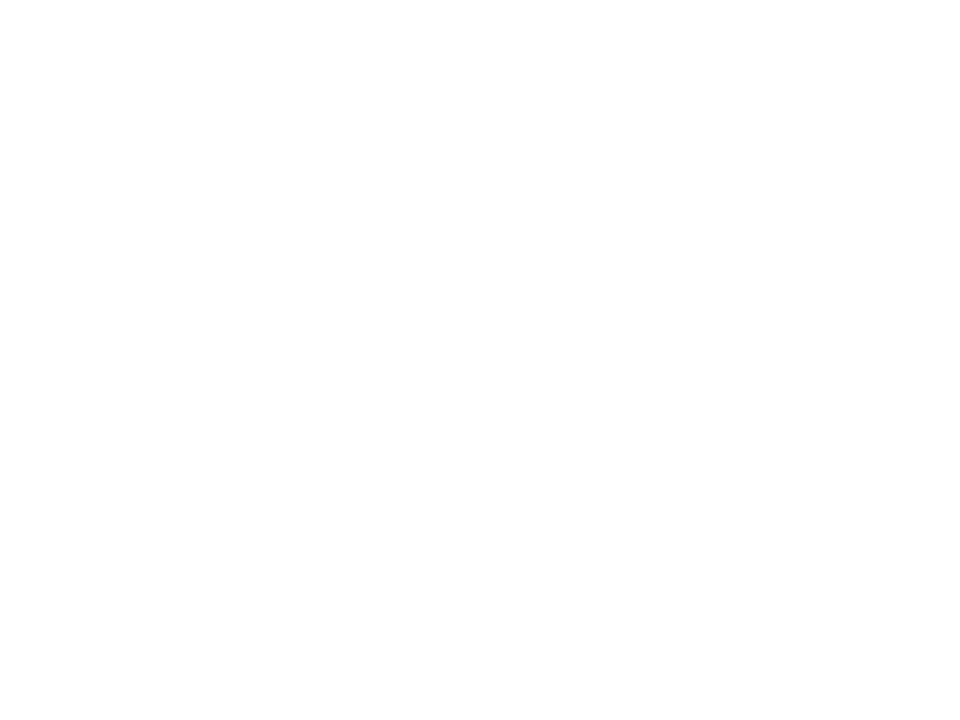
\includegraphics[width=\textwidth]{figs/batch32_lr0.1.pdf}
        \caption[]%
        {{\small Network 2}}    
        \label{fig:mean and std of net24}
    \end{subfigure}
    \vskip\baselineskip
    \begin{subfigure}[b]{0.475\textwidth}   
        \centering 
        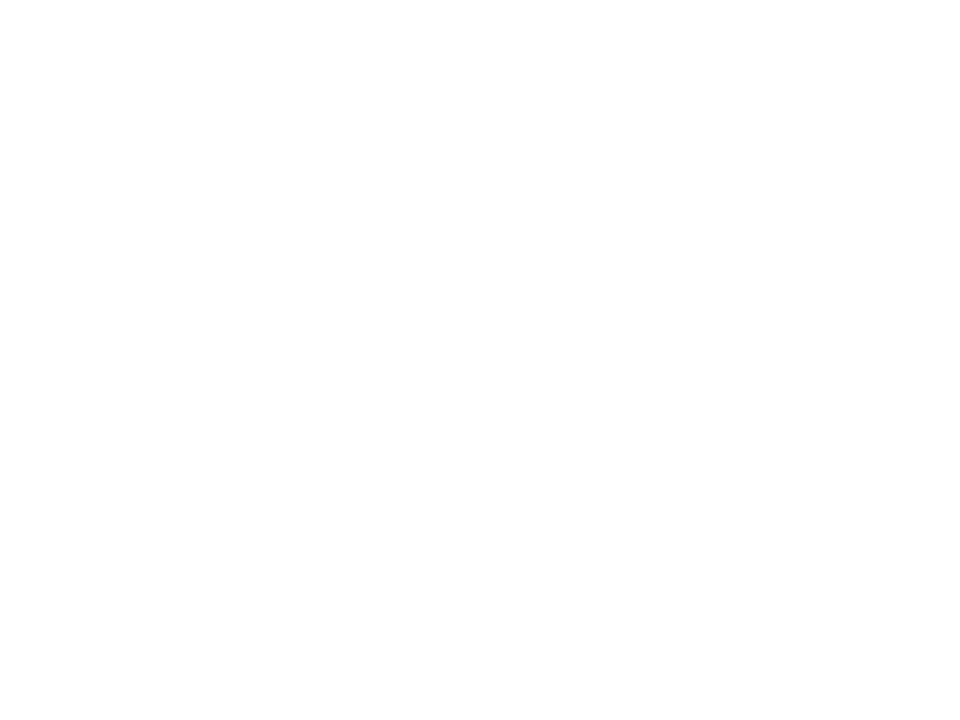
\includegraphics[width=\textwidth]{figs/batch32_lr0.1.pdf}
        \caption[]%
        {{\small Network 3}}    
        \label{fig:mean and std of net34}
    \end{subfigure}
    \hfill
    \begin{subfigure}[b]{0.475\textwidth}   
        \centering 
        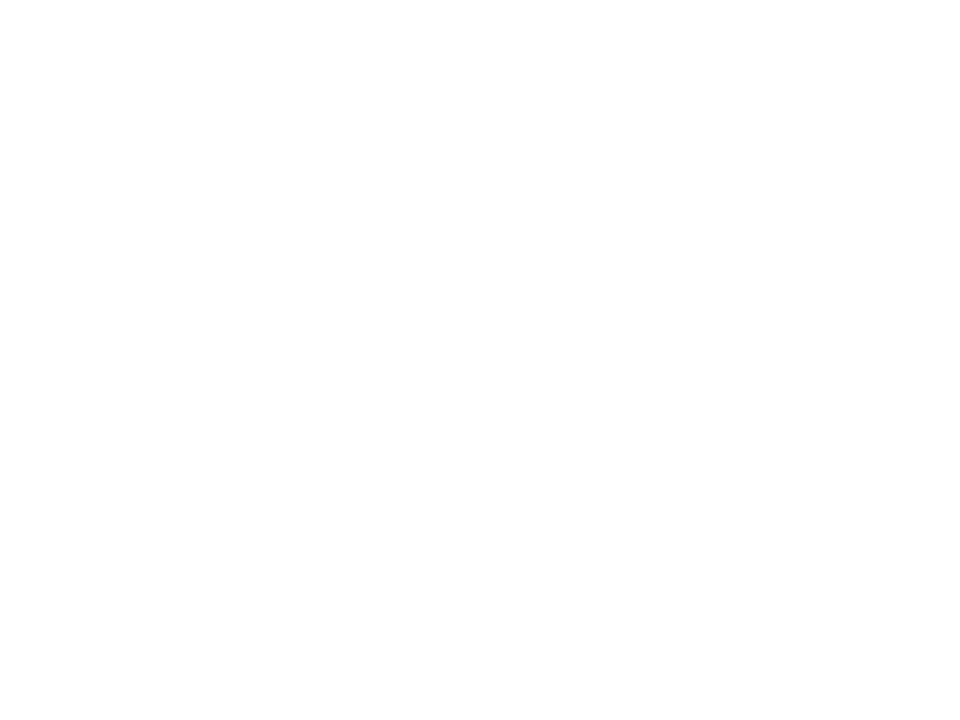
\includegraphics[width=\textwidth]{figs/batch32_lr0.1.pdf}
        \caption[]%
        {{\small Network 4}}    
        \label{fig:mean and std of net44}
    \end{subfigure}
    \caption[ The average and standard deviation of critical parameters ]
    {\small The average and standard deviation of critical parameters: Region R4} 
    \label{fig:mean and std of nets}
\end{figure*}

\paragraph{17. What is the error at the start of the first epoch, in train and test? How can you interpret this?}
The accuracy on the test set is better that the accuracy on train. It's because. 
We must be aware that the training loss and accuracy is calculated \textbf{at every batch} so before the end of the first epoch, parameters and so result (loss and accuracy) are variating a lot. It mean that at the first batch of the first epoch we take into account the loss calculated only with \textit{batch\_size} examples.

Contrary to the test loss and accuracy that are computed at the end of the first epoch, after the model have seen all training example. Those value are more true that those from train at the first epoch % pire phrase

\paragraph{18. $ \bigstar $ Interpret the results. What's wrong? What is this phenomenon?}
We observe overfitting. We can see that starting from epoch three or four that our accuracy on test cross the curve of the accuracy of train. It mean that we are becoming better on train sample but worse on the test sample. The model can't generalize on new image.


\subsection{Results improvements}
\subsubsection{Standardization of examples}
\paragraph{19. Describe your experimental results.}

\paragraph{20. Why only calculate the average image on the training examples and normalize the validation examples with the same image?}

\paragraph{21. Bonus : There are other normalization schemes that can be more efficient like ZCA normalization. Try other methods, explain the differences and compare them to the one requested.}

\subsubsection{Increase in the number of training examples by \textit{data increase}}
\paragraph{22. Describe your experimental results and compare them to previouscrease results.}

\paragraph{23. Does this horizontal symmetry approach seems usable on all types of images? In what cases can it be or not be?}

\paragraph{24. What limits do you see in this type of data increase by transformation of the dataset?}

\subsubsection{Variants of the optimization algorithm}
\paragraph{26. Describe your experimental results and compare them to previous results, including learning stability.}

\paragraph{27. Why does this method improve learning?}


\subsubsection{Regularization of the network by \textit{dropout}}
\paragraph{29. Describe your experimental results and compare them to previous results.}

\paragraph{30. What is regularization in general?}

\paragraph{31. Research and "discuss" possible interpretations of the effect of dropout on the behavior of a network using it?}

\paragraph{32. What is the influence of the hyperparameter of this layer?}

\paragraph{33. What is the difference in behavior of the dropout layer between training and test?}

\subsubsection{Use of \textit{batch normalization}}

\paragraph{34. Describe your experimental results and compare them to previous results.}

\end{document}